\documentclass[12pt]{article}
\usepackage[a4paper, margin=2cm]{geometry} %Annina style
\usepackage[utf8]{inputenc}
\usepackage{graphicx}
\usepackage{amsmath}
\usepackage{amsfonts}
\usepackage{amssymb}
\usepackage{hyperref}
\usepackage{setspace} % Add this package for spacing commands
\usepackage[numbers]{natbib} % Add this package for bibliography management
\usepackage{float}
\usepackage{listings}
\usepackage{xcolor}
\usepackage{caption} % Required for using \captionof

\renewcommand{\lstlistingname}{Code}
\lstset{ 
    language=Python, 
    basicstyle=\ttfamily\small, 
    keywordstyle=\color{blue}, 
    stringstyle=\color{red}, 
    commentstyle=\color{green}, 
    showstringspaces=false,
    numbers=left,
    numberstyle=\tiny\color{gray},
    frame=single,
    breaklines=true
}
\setlength{\parindent}{0pt}

\title{XAI: Cluster Variational Inference Notes}
\author{Jack Li}
\date{October 2023}

\begin{document}

\maketitle

\begin{abstract}
\ldots


\end{abstract}

\section{Workflow}

Variational Inference model explanation\\
The purpose of this report is to introduce the Variational Inference Cluster algorithm and experiment with it. \\

Situations:\\
1. ML model interpretability is attracting more attention in order to improve model performance and robustness in industrial applications.\\
2. Briefly outline the importance of machine learning insterpretability in the medical field, financial field, and autonomous driving. Explainable AI and adversarial attacks highlight the importance of understanding models.\\
3. Explainable AI (XAI) aims to understand the model's decision-making process.\\
4. Adversarial attacks exploit key features to influence the output.\\

Problem:\\
1. Applying the model in the wrong field.\\
2. The model outputs something incorrect, and people are not able to understand why.\\
3. Users blindly trust the model.\\
4. Do XAI and adversarial attack techniques share the same results?\\

Solution:\\
1. Examine and compare state-of-the-art techniques.\\
2. Use Variational Inference for model explanation.\\

Evaluation:\\
Show the comparison of results.\\


\section{Introduction}

Machine learning encompasses a variety of tasks, including classification, segmentation, and modern techniques such as generative models. 
One fundamental aspect of machine learning is classification, which involves categorizing data into labeled and unlabeled datasets. 
This process includes techniques from both supervised and unsupervised learning. 
A key feature of unsupervised learning is clustering, an algorithm designed to group data into distinct clusters based on inherent similarities.
Clustering is an unsupervised learning technique aimed at partitioning data into different clusters. 
One of the significant challenges in this field is the difficulty in understanding how models work analytically, which can lead to unpredictable results in critical applications such as medical diagnosis, financial fraud detection, and autonomous driving. 
Therefore, understanding model interpretability for key features is crucial. This is where the concept of explainable AI (XAI) becomes relevant. 
XAI is a subfield of artificial intelligence focused on making AI models more transparent and understandable to humans. \\

Another important area of research is adversarial attacks, which further underscores the importance of XAI and the need to comprehend model behavior. 
While XAI aims to elucidate the model's decision-making process, adversarial attacks seek to exploit the model's vulnerabilities.\cite{Athalye2018} \cite{Moosavi-Dezfooli2017}
The robustness of models is crucial for their real-world applications, and understanding the dynamics between XAI and adversarial attacks is essential for improving model interpretability and reliability. 
Despite their differences, both fields highlight the necessity of understanding AI models.\\

In this paper, we explore state-of-the-art techniques in explainable AI (XAI) and adversarial attacks, focusing on how they interpret features in images differently. 
Through our exploration, we found that images in high-dimensional spaces significantly contribute to model complexity. This complexity aligns with the challenges posed by both XAI and adversarial attacks. Specifically, while XAI aims to elucidate the decision-making process of complex models, adversarial attacks exploit the vulnerabilities inherent in these high-dimensional representations. Understanding these dynamics is crucial for improving model robustness and interpretability.
As we advocate for the idea of XAI, we introduce the Variational Inference Clustering algorithm and experiment with it. 
This algorithm is a popular XAI method used to interpret features in images.



\section{Related Work}
\ldots

In this paper, we explore state-of-the-art XAI and adversarial attack techniques and how they interpret features in images differently. 
From the foundations of machine learning and deep learning, we know that improved predictive accuracy often comes with increased model complexity. 
This complexity can decrease the in-sample error ($E_{in}$) but may increase the out-of-sample error ($E_{out}$) \cite{Shalev-Shwartz2014, Devroye1996, Hastie2017}. 
To better understand models, it is essential to interfere with their decision-making processes.

The GradCAM\cite{Selvaraju2020}, algorithm is a popular XAI algorithm. 
\section{Experiments}
\ldots
VI Structures:\\

The variational inference algorithm is a popular XAI method used to interpret features in images.
The clusters example\cite{Blei2017} \\

Formulation:
\begin{align} 
  \begin{split}
z_j & \sim \mathcal{N}(m^2, s^2)~\text{for } j = 1, ..., K \\\\
c_i & \sim \mathcal{U}(K)~\text{for } i = 1, ..., N \\\\ 
x_i & \sim \mathcal{N}(c_i^T \mu, 1)~\text{for} i = 1, ..., N \\\\
y  & \sim CNN
  \end{split}
\end{align}

ELBO function:
\begin{align}
ELBO & = E_q[log~p(x,\hat{z})] - E_q[log~q(\hat{z})]\\
 &= E_q[log~p(x,z,c,y) - log~q(z,c,y)]
\end{align}

Encoder $q(.)$:


\begin{align}
  \begin{split}
log~ q(z,c,y) &= log~[q(z|m, s^2)~q(c| \phi)~q(y|z,c)] \\\\
 &= log~\left[ \prod_j q(z_{j}| m_j, s_j^2)~\prod_i q(c_i| \phi_i)~q(y| z,c) \right]\\\\
&= \sum_{j}~\log~q(z_{j}| m_j, s_j^2) +  \sum_{j} \log~ \phi_{j} + \log~ \text{pred}_{y} \\ \\
&\propto \sum_{j}~ \frac{-1}{2}\left( \log~s^2 + \frac{(z_{j}-m_{j})^2}{s_{j}^2} \right)+\sum_{j} \log~ \phi_{j} + \log~ \text{pred}_{y}
  \end{split}
\end{align}

Decoder $p(.)$:


$$p(c_i) = \dfrac{1}{K}$$

$$p(y) = N(y|0,1)$$

\begin{align*}
log~p(x_i~\vert~c_i, z_{j},y) &= log~\prod_j p(x_i~\vert~z_j ,~y)^{c_{ij}} \prod_{j}~p(c,z|y) ~p(y)\\ \\
 &\propto \sum_j c_{j} log~p(x_i~\vert~z_j)~\sum_{j}c_{j}\log\left( -\frac{1}{2\pi}e^{-\frac{1}{2}\left( \frac{z_{j}-\mu_{y}}{1} \right)^2} \right) \\ \\
 &\propto \sum_j c_{j} log~p(x_i~\vert~z_j)  -\frac{1}{2}~\sum_{j}c_{j}\left( \frac{z_{j}-\mu_{y}}{1} \right)^2 \\ \\ \\
&\propto -\frac{1}{2}( \sum_j c_{j}\left( \frac{x_{i}-m_{j}}{1} \right)^2+~\sum_{j}c_{j}\left( \frac{z_{j}-\mu_{y}}{1} \right)^2)
\end{align*}


\begin{align*}
ELBO  &= E_q[log~p(x,z,c,y) - log~q(z,c,y)] \\ \\
&= E_{q}[-\frac{1}{2}( \sum_j c_{j}\left( x_{i}-m_{j} \right)^2+~\sum_{j}c_{j}\left( z_{j}-\mu_{y} \right)^2) + \frac{1}{2}\left(\sum_{j} \log~s^2  \right) - \sum_{j} \log~ \phi_{j} - \log~ \text{pred}_{y}] \\ \\
\end{align*}



\subsection{Full Connected Variational Inference}

\begin{figure}[H]
    \centering
    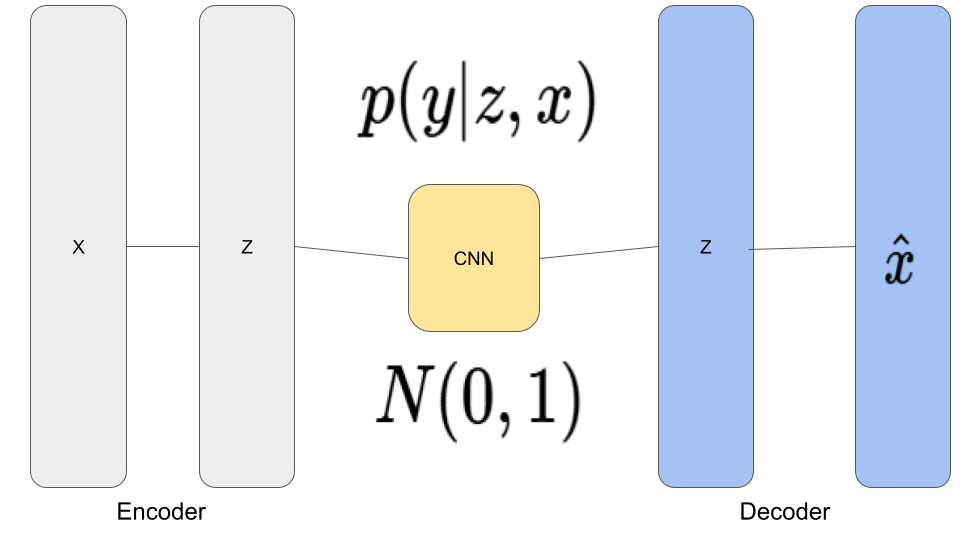
\includegraphics[width=0.5\linewidth]{../fig/Full connected Variational Inference.png} % Replace with the path to your image
    \caption{Using 784 $z=\{ \mu,s \}$ }
    \label{fig:full_connected}
\end{figure}


  \begin{lstlisting}[language=Python, caption= Full connected VI loss function]
def loss_elbo(x, mu, log_var, phi, x_recon, model, predicted):
    # HACK: use the CNN model predition as the input
    t1 = 0.5 * (mu.view(1, -1) - mu_y.view(-1, 1)) ** 2
    t1 = phi * t1
    t1 = -t1.mean()

    # NOTE: Alternative implementation
    t2 = 0.5 * (x - x_recon) ** 2
    t2 = phi * t2
    t2 = torch.mean(t2)

    t3 = 0.5 * log_var.exp().mean()

    t4 = -torch.log(phi + 1e-10).mean()

    # HACK: use the CNN model predition as the input
    model.eval()
    input = x_recon.view(1, 1, 28, 28)
    # Forward pass
    outputs = model(input)
    outputs = F.softmax(outputs, dim=1)
    outputs = torch.clamp(outputs, 1e-10, 1 - 1e-10)
    t5 = -torch.log(outputs[:, predicted])
    return -(t1 + t2 + t3 + t4 + t5) + lamb
\end{lstlisting}

\begin{figure}[H]
    \centering
    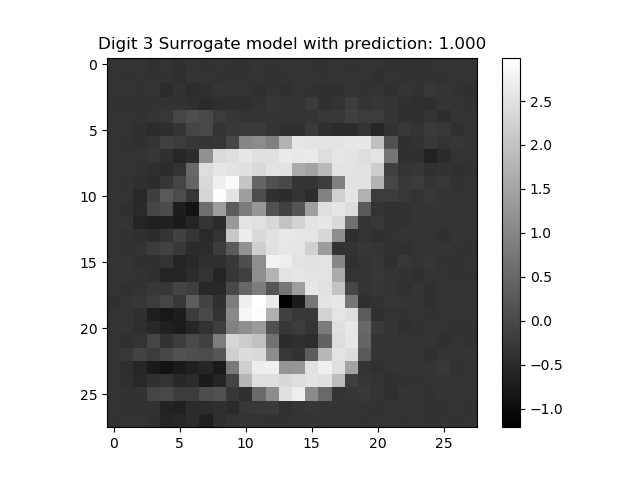
\includegraphics[width=0.7\linewidth]{../fig/ID 3-Digit 8 pred 3 new_image.png} % Replace with the path to your image
    \caption{MNIST Prediction with 784 $z=\{\mu,s \}$ }
    \label{fig:naive_bayes}
\end{figure}

\subsection{Conv2d Variational Inference}
\begin{figure}[H]
    \centering
    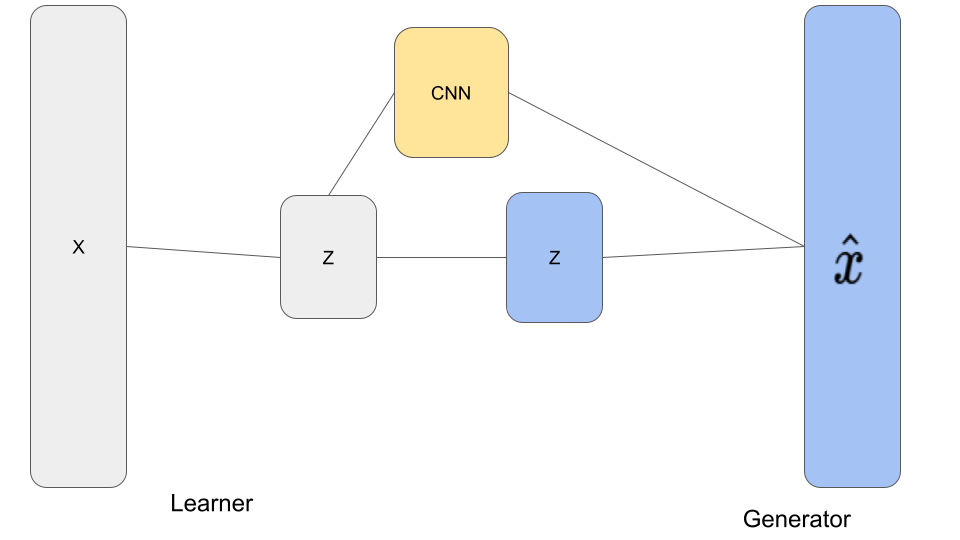
\includegraphics[width=0.5\linewidth]{../fig/GANandVAE.png} % Replace with the path to your image
    \caption{Using GAN and VAE method with conv2d }
    \label{fig:GANandVAE}
\end{figure}


\begin{figure}[H]
    \centering
    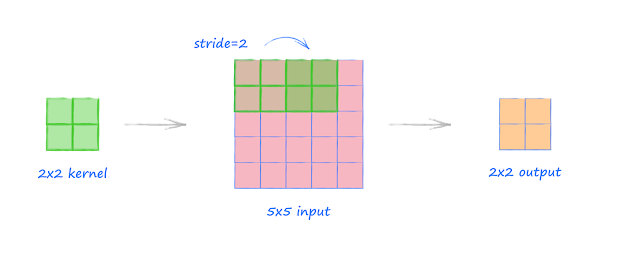
\includegraphics[width=0.5\linewidth]{../fig/2x2kernelstrike2.png} % Replace with the path to your image
    \caption{use conv2d kernel size 2x2 and stride 2}
    \label{fig:conv2d}
\end{figure}

\begin{lstlisting}[language=Python, caption= GAN and VAE model]
  class generator(nn.Module):
    def __init__(self, channels_img):
        super().__init__()
        self.channels_img = channels_img
        # self.features_d = features_d
        self.k = 2
        # decoder
        self.decoder = nn.Sequential(
            # NOTE: convTranspose2d output = (input -1)*s -2p + k + op
            # (14-1)*2 + 2 = img 28x28
            nn.ConvTranspose2d(
                channels_img, channels_img, kernel_size=2, stride=2, padding=0
            ),
            nn.Tanh(),
        )

        self.p_layer = nn.Sequential(
            # NOTE: convTranspose2d output = (input -1)*s -2p + k + op
            # (14-1)*2 + 2 = img 28x28
            nn.ConvTranspose2d(
                channels_img, channels_img * self.k, kernel_size=2, stride=2, padding=0
            ),
            nn.Tanh(),
        )

    def forward(self, x, z):
        p = self.p_layer(z)
        p = F.softmax(p, dim=0)
        # x_recon = self.decoder(z) * p[:, 0, :, :] + x * (p[:, 1, :, :])
        x_recon = self.decoder(z)
        return x_recon, p


class learner(nn.Module):
    def __init__(self, channels_img):
        super().__init__()
        self.channels_img = channels_img
        # self.features_d = features_d
        self.k = 2
        # encoder
        # latent mean and variance
        self.mean_layer = nn.Sequential(
            # NOTE: conv2d output = (input + 2p -k)/s +1
            # (28-2)/2 +1 = img 14x14
            nn.Conv2d(channels_img, channels_img, kernel_size=2, stride=2),
            nn.InstanceNorm2d(channels_img, affine=True),
            nn.LeakyReLU(0.2),
        )  # latent mean and variance
        self.logvar_layer = nn.Sequential(
            # NOTE: conv2d output = (input + 2p -k)/s +1
            # (28-2)/2 +1 = img 14x14
            nn.Conv2d(channels_img, channels_img, kernel_size=2, stride=2),
            nn.InstanceNorm2d(channels_img, affine=True),
            nn.LeakyReLU(0.2),
        )

    def reparameterization(self, mean, var):
        # mean = mean.view(mean.size[0], -1)
        # var = var.view(var.size[0], -1)
        epsilon = torch.randn_like(var).to(device)
        z = mean + var * epsilon
        return z

    def encode(self, x):
        mean, logvar = self.mean_layer(x), self.logvar_layer(x)
        return mean, logvar

    def forward(self, x):
        mean, log_var = self.encode(x)
        z = self.reparameterization(mean, log_var)
        return z, mean, log_var

\end{lstlisting}

\begin{lstlisting}[language=Python, caption= GAN and VAE loss function]
epochs = 1000
leaner_epochs = 10
predicted = true_y
# predicted = 9
G = generator(1).to(device)
L = learner(1).to(device)

opt_G = torch.optim.Adam(G.parameters(), lr=0.005)
opt_L = torch.optim.Adam(L.parameters(), lr=0.005)


def loss_function(x, x_recon, mean, log_var, p):
    alpha = torch.sum(p[:, 0, :, :])
    # reproduction_loss = F.mse_loss(x_recon * p[:, 0, :, :], x * p[:, 0, :, :])
    reproduction_loss = F.mse_loss(x_recon, x)
    KLD = -0.5 * torch.sum(1 + log_var - mean.pow(2) - log_var.exp())

    return reproduction_loss + KLD


# %%

for epoch in range(epochs + 1):
    for leaner_epoch in range(leaner_epochs + 1):
        opt_L.zero_grad()
        x = img.clone().to(device)
        x = x.view(1, 1, 28, 28)
        z, mean, log_var = L(x)
        x_recon, p = G(x, z)
        # Get the index of the max log-probability
        model.eval()
        critic_fake = F.softmax(model(x_recon), dim=1)[0][predicted]

        loss_L = -(torch.mean(critic_fake))
        # loss = loss_function(x, x_recon, mean, log_var) - torch.log(critic_real + 1e-5) * (
        #     -torch.log(critic_fake + 1e-5)
        # )

        loss_L.backward(retain_graph=True)
        opt_L.step()

    opt_G.zero_grad()
    x = img.clone().to(device)
    x = x.view(1, 1, 28, 28)
    z, mean, log_var = L(x)
    x_recon, p = G(x, z)

    model.eval()
    critic_fake = F.softmax(model(x_recon), dim=1)[0][predicted]
    t1 = -torch.sum(torch.log(critic_fake + 1e-5))
    t2 = loss_function(x, x_recon, mean, log_var, p)

    # NOTE: original loss function
    loss_G = t1 + t2
    # NOTE: alternative loss function, from GAN
    # loss_G = torch.mean(critic_fake)

    loss_G.backward()
    opt_G.step()
\end{lstlisting}

\begin{table}[H]
    \centering
    \caption{Experiments Comparison table with top n-th variance(v3)}
    \begin{tabular}{|c|c|}
        \hline
        
        \hline
        \begin{minipage}{0.45\linewidth}
            \centering

            n = 5 \\
            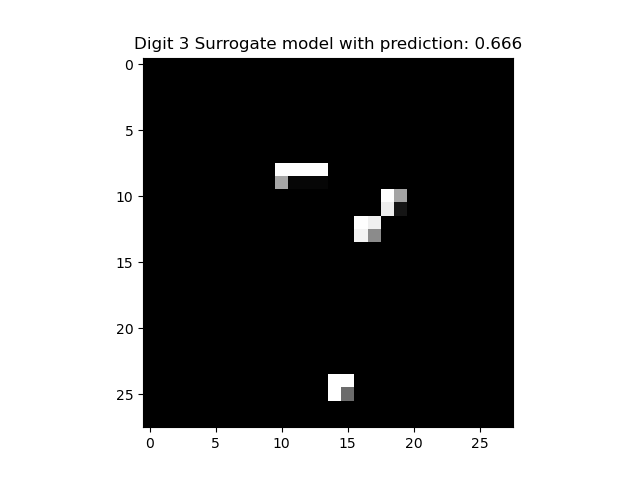
\includegraphics[width=\linewidth]{../fig/ID 3-Digit 8 pred 3 with n=5.png}
        \end{minipage} &
        \begin{minipage}{0.45\linewidth}
            \centering

            n = 5
            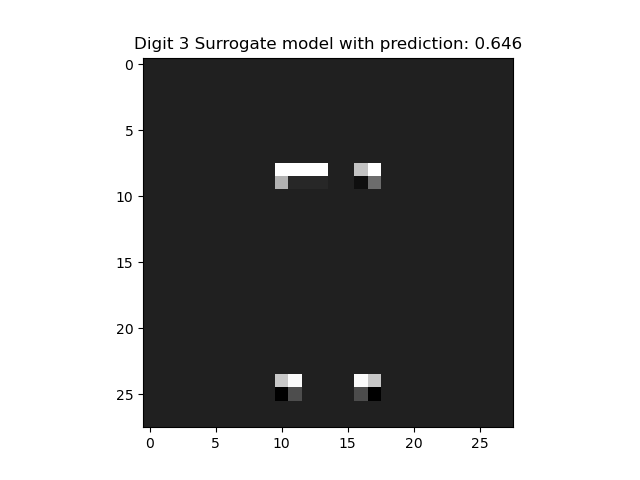
\includegraphics[width=\linewidth]{../fig/ID 3-Digit 8 pred 3 with n=5-1_1.png}
        \end{minipage} \\
        \\
        \hline
        \begin{minipage}{0.45\linewidth}
            \centering

            n = 10 \\
            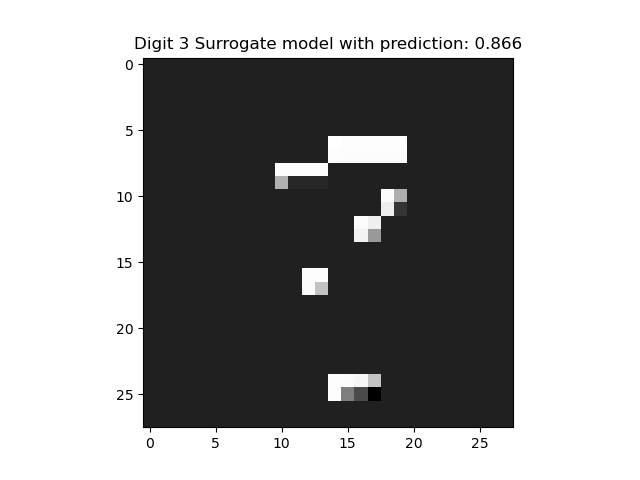
\includegraphics[width=\linewidth]{../fig/ID 3-Digit 8 pred 3 with n=10.png}
        \end{minipage} &
        \begin{minipage}{0.45\linewidth}
            \centering

            n = 10
            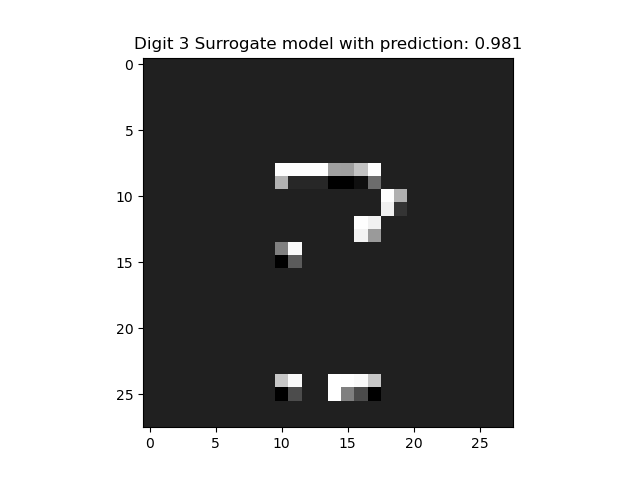
\includegraphics[width=\linewidth]{../fig/ID 3-Digit 8 pred 3 with n=10-1_1.png}
        \end{minipage} \\
        \\
        \hline
        \begin{minipage}{0.45\linewidth}
            \centering

            n = 12 \\
            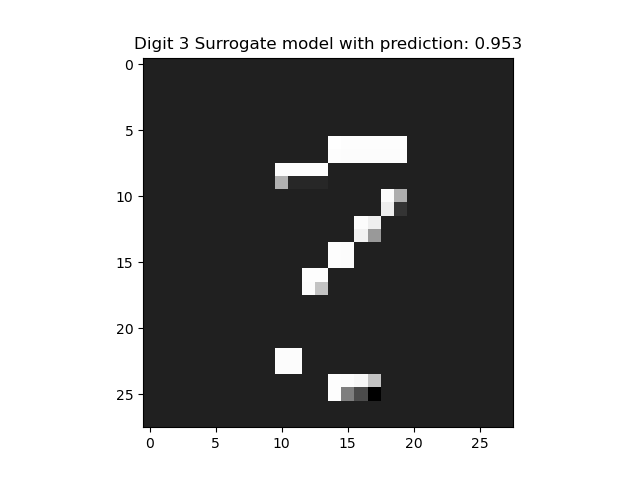
\includegraphics[width=\linewidth]{../fig/ID 3-Digit 8 pred 3 with n=12.png}
        \end{minipage} &
        \begin{minipage}{0.45\linewidth}
            \centering

            n = 12
            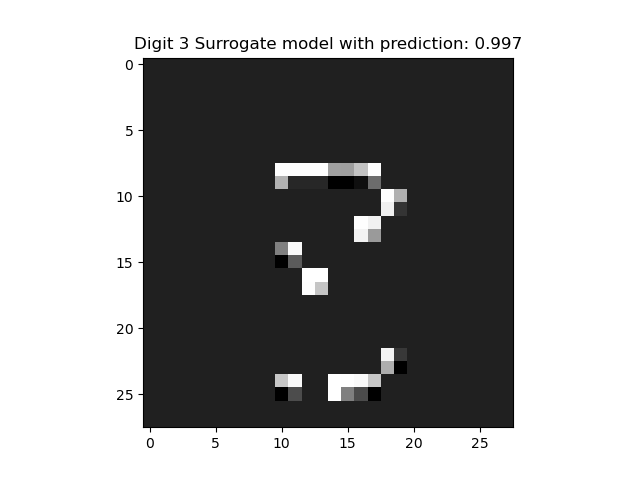
\includegraphics[width=\linewidth]{../fig/ID 3-Digit 8 pred 3 with n=12-1_1.png}
        \end{minipage} \\
        \\
        \hline
        \begin{minipage}{0.45\linewidth}
            \centering

            n = 13 \\
            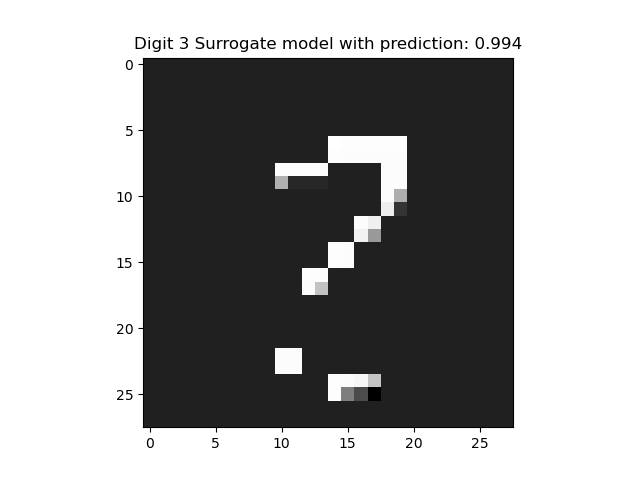
\includegraphics[width=\linewidth]{../fig/ID 3-Digit 8 pred 3 with n=13.png}
        \end{minipage} &
        \begin{minipage}{0.45\linewidth}
            \centering

            n = 13
            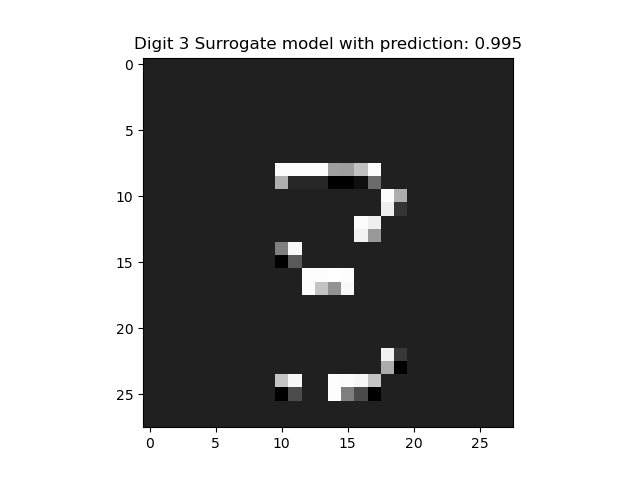
\includegraphics[width=\linewidth]{../fig/ID 3-Digit 8 pred 3 with n=13-1_1.png}
        \end{minipage} \\
        \\
        \hline
    \end{tabular}
    \label{tab:example}
\end{table}

\newpage
\begin{table}[H]
    \centering
    \caption{Experiments Comparison table with top n-th variance(v3)}
    \begin{tabular}{|c|c|}
        \hline
        \begin{minipage}{0.45\linewidth}
            \centering

            n = 15 \\
            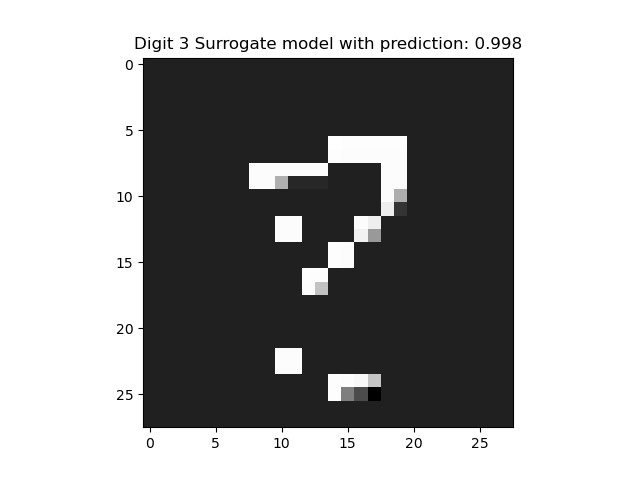
\includegraphics[width=\linewidth]{../fig/ID 3-Digit 8 pred 3 with n=15.png}
        \end{minipage} &
        \begin{minipage}{0.45\linewidth}
            \centering

            n = 15
            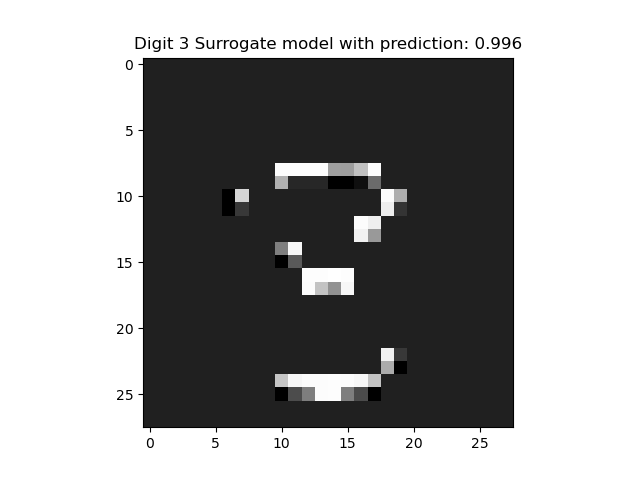
\includegraphics[width=\linewidth]{../fig/ID 3-Digit 8 pred 3 with n=15-1_1.png}
        \end{minipage} \\
        \\
        \hline
        \begin{minipage}{0.45\linewidth}
            \centering

            n = 20 \\
            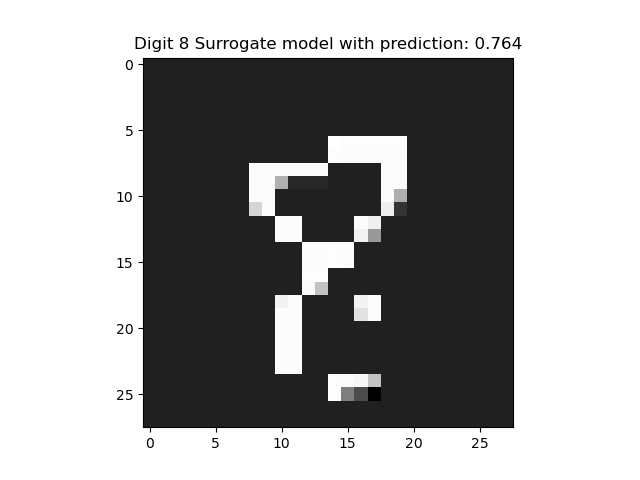
\includegraphics[width=\linewidth]{../fig/ID 3-Digit 8 pred 8 with n=20.png}
        \end{minipage} &
        \begin{minipage}{0.45\linewidth}
            \centering

            n = 20
            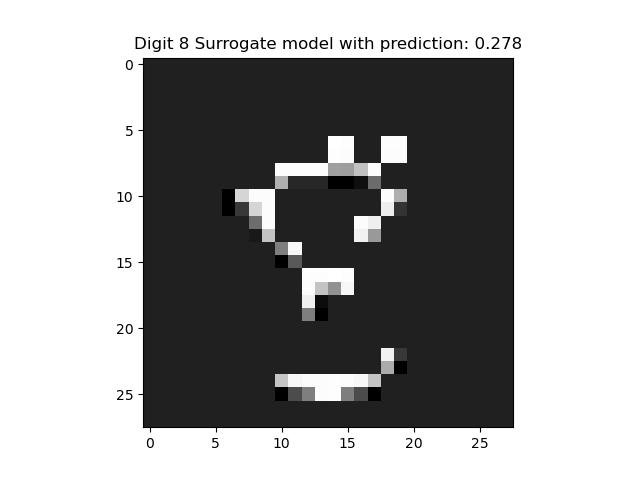
\includegraphics[width=\linewidth]{../fig/ID 3-Digit 8 pred 8 with n=20-1_1.png}
        \end{minipage} \\
        \\
        \hline
        \begin{minipage}{0.45\linewidth}
            \centering

            n = 25 \\
            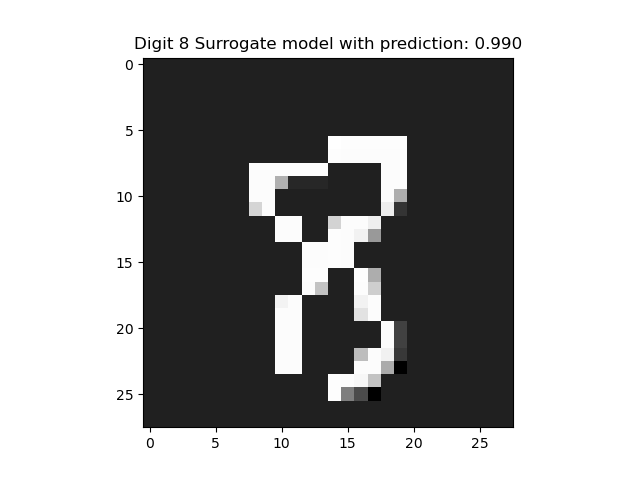
\includegraphics[width=\linewidth]{../fig/ID 3-Digit 8 pred 8 with n=25.png}
        \end{minipage} &
        \begin{minipage}{0.45\linewidth}
            \centering

            n = 25
            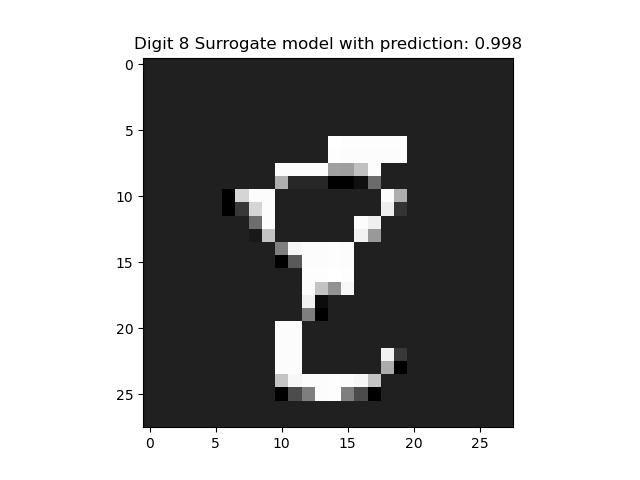
\includegraphics[width=\linewidth]{../fig/ID 3-Digit 8 pred 8 with n=25-1_1.png}
        \end{minipage} \\
        \\
        \hline
        \begin{minipage}{0.45\linewidth}
            \centering

            n = 30 \\
            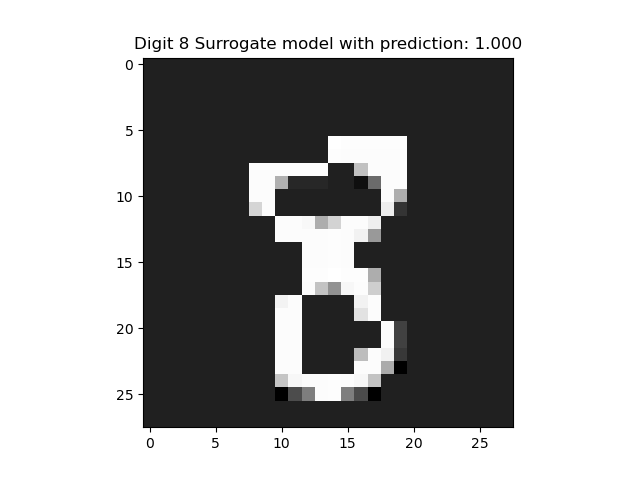
\includegraphics[width=\linewidth]{../fig/ID 3-Digit 8 pred 8 with n=30.png}
        \end{minipage} &
        \begin{minipage}{0.45\linewidth}
            \centering

            n = 30
            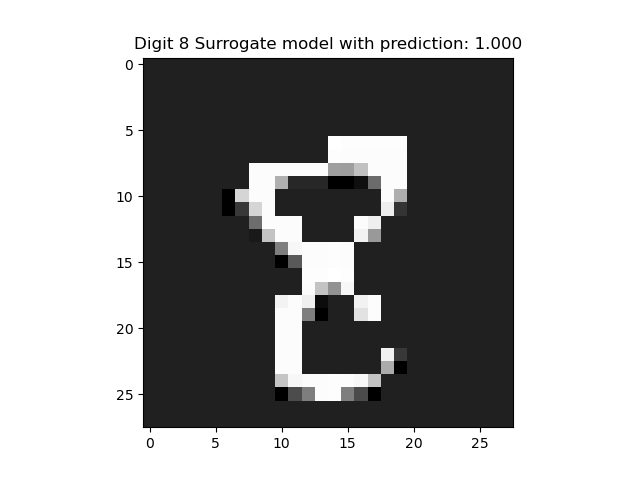
\includegraphics[width=\linewidth]{../fig/ID 3-Digit 8 pred 8 with n=30-1_1.png}
        \end{minipage} \\
        \\
        \hline
    \end{tabular}
    \label{tab:example}
\end{table}

\newpage
\begin{table}[H]
    \centering
    \caption{Train one class Experiments Comparison table with mask $C < 0.1$ (v4)}
    \begin{tabular}{|c|c|}
        \hline
        \begin{minipage}{0.45\linewidth}
            \centering

            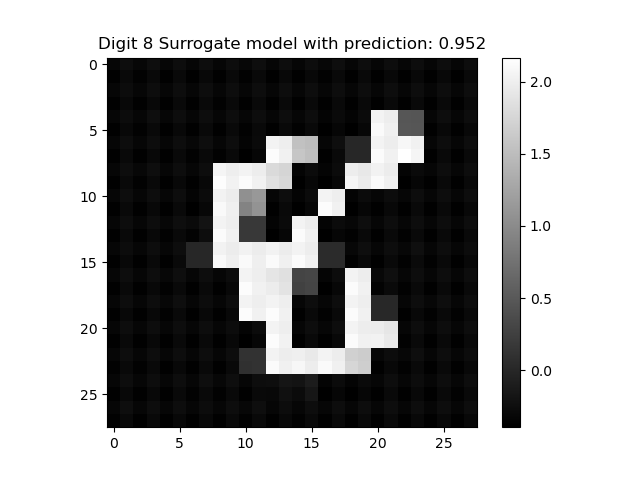
\includegraphics[width=\linewidth]{../fig/ID 1-Digit 8 pred 8 new_image.png}
        \end{minipage} &
        \begin{minipage}{0.45\linewidth}
            \centering

            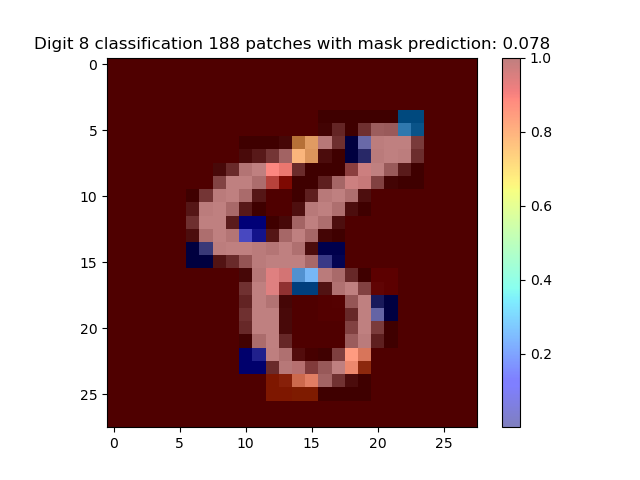
\includegraphics[width=\linewidth]{../fig/ID 1-Digit 8 classification n patches = 188.png}
        \end{minipage} \\
        \\
        \hline
        \begin{minipage}{0.45\linewidth}
            \centering

            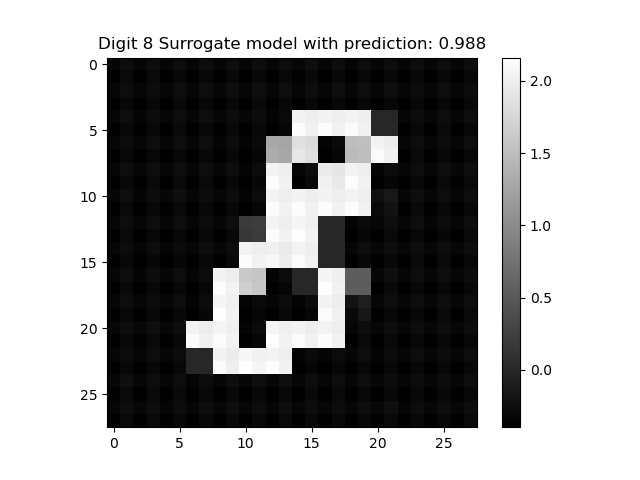
\includegraphics[width=\linewidth]{../fig/ID 2-Digit 8 pred 8 new_image.png}
        \end{minipage} &
        \begin{minipage}{0.45\linewidth}
            \centering

            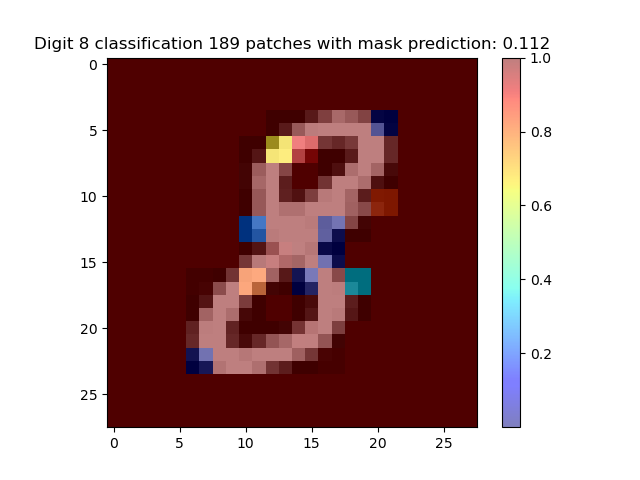
\includegraphics[width=\linewidth]{../fig/ID 2-Digit 8 classification n patches = 189.png}
        \end{minipage} \\
        \\
        \hline
        \begin{minipage}{0.45\linewidth}
            \centering

            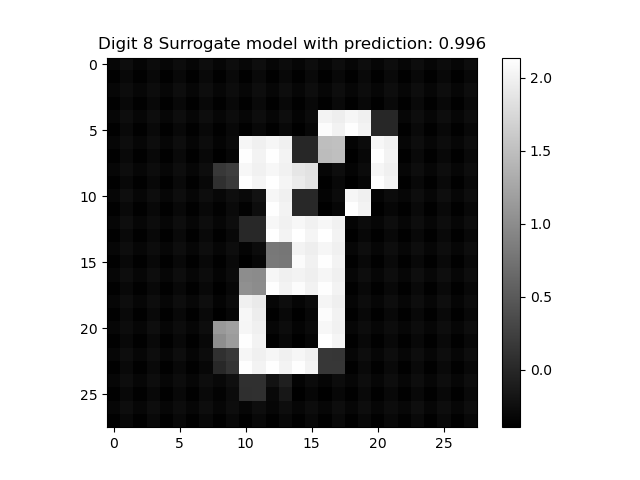
\includegraphics[width=\linewidth]{../fig/ID 4-Digit 8 pred 8 new_image.png}
        \end{minipage} &
        \begin{minipage}{0.45\linewidth}
            \centering

            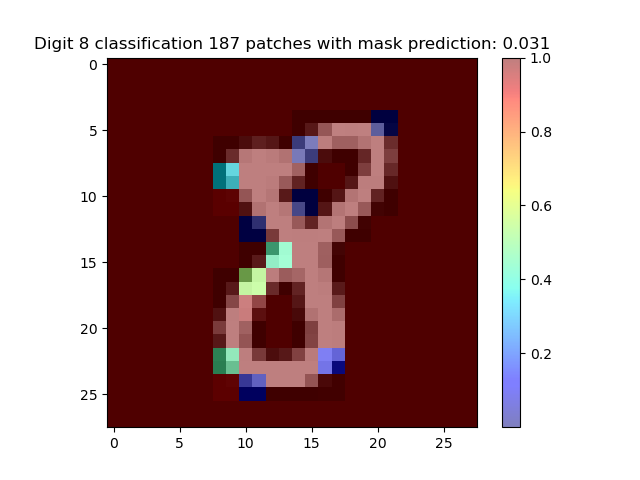
\includegraphics[width=\linewidth]{../fig/ID 4-Digit 8 classification n patches = 187.png}
        \end{minipage} \\
        \\
        \hline
        \begin{minipage}{0.45\linewidth}
            \centering

            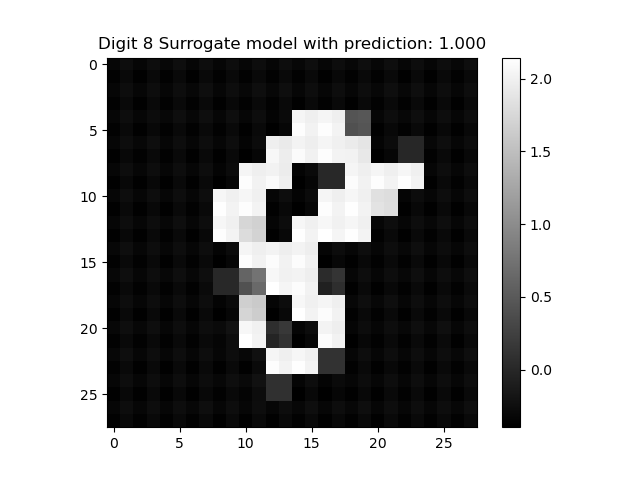
\includegraphics[width=\linewidth]{../fig/ID 5-Digit 8 pred 8 new_image.png}
        \end{minipage} &
        \begin{minipage}{0.45\linewidth}
            \centering

            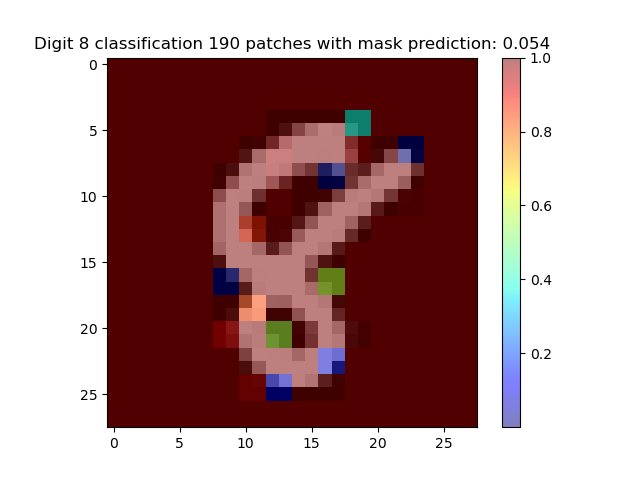
\includegraphics[width=\linewidth]{../fig/ID 5-Digit 8 classification n patches = 190.png}
        \end{minipage} \\
        \\
        \hline
    \end{tabular}
    \label{tab:example}
\end{table}


\section{Future Work}


Sharingan Evolution:\\

\begin{figure}[H]
    \centering
    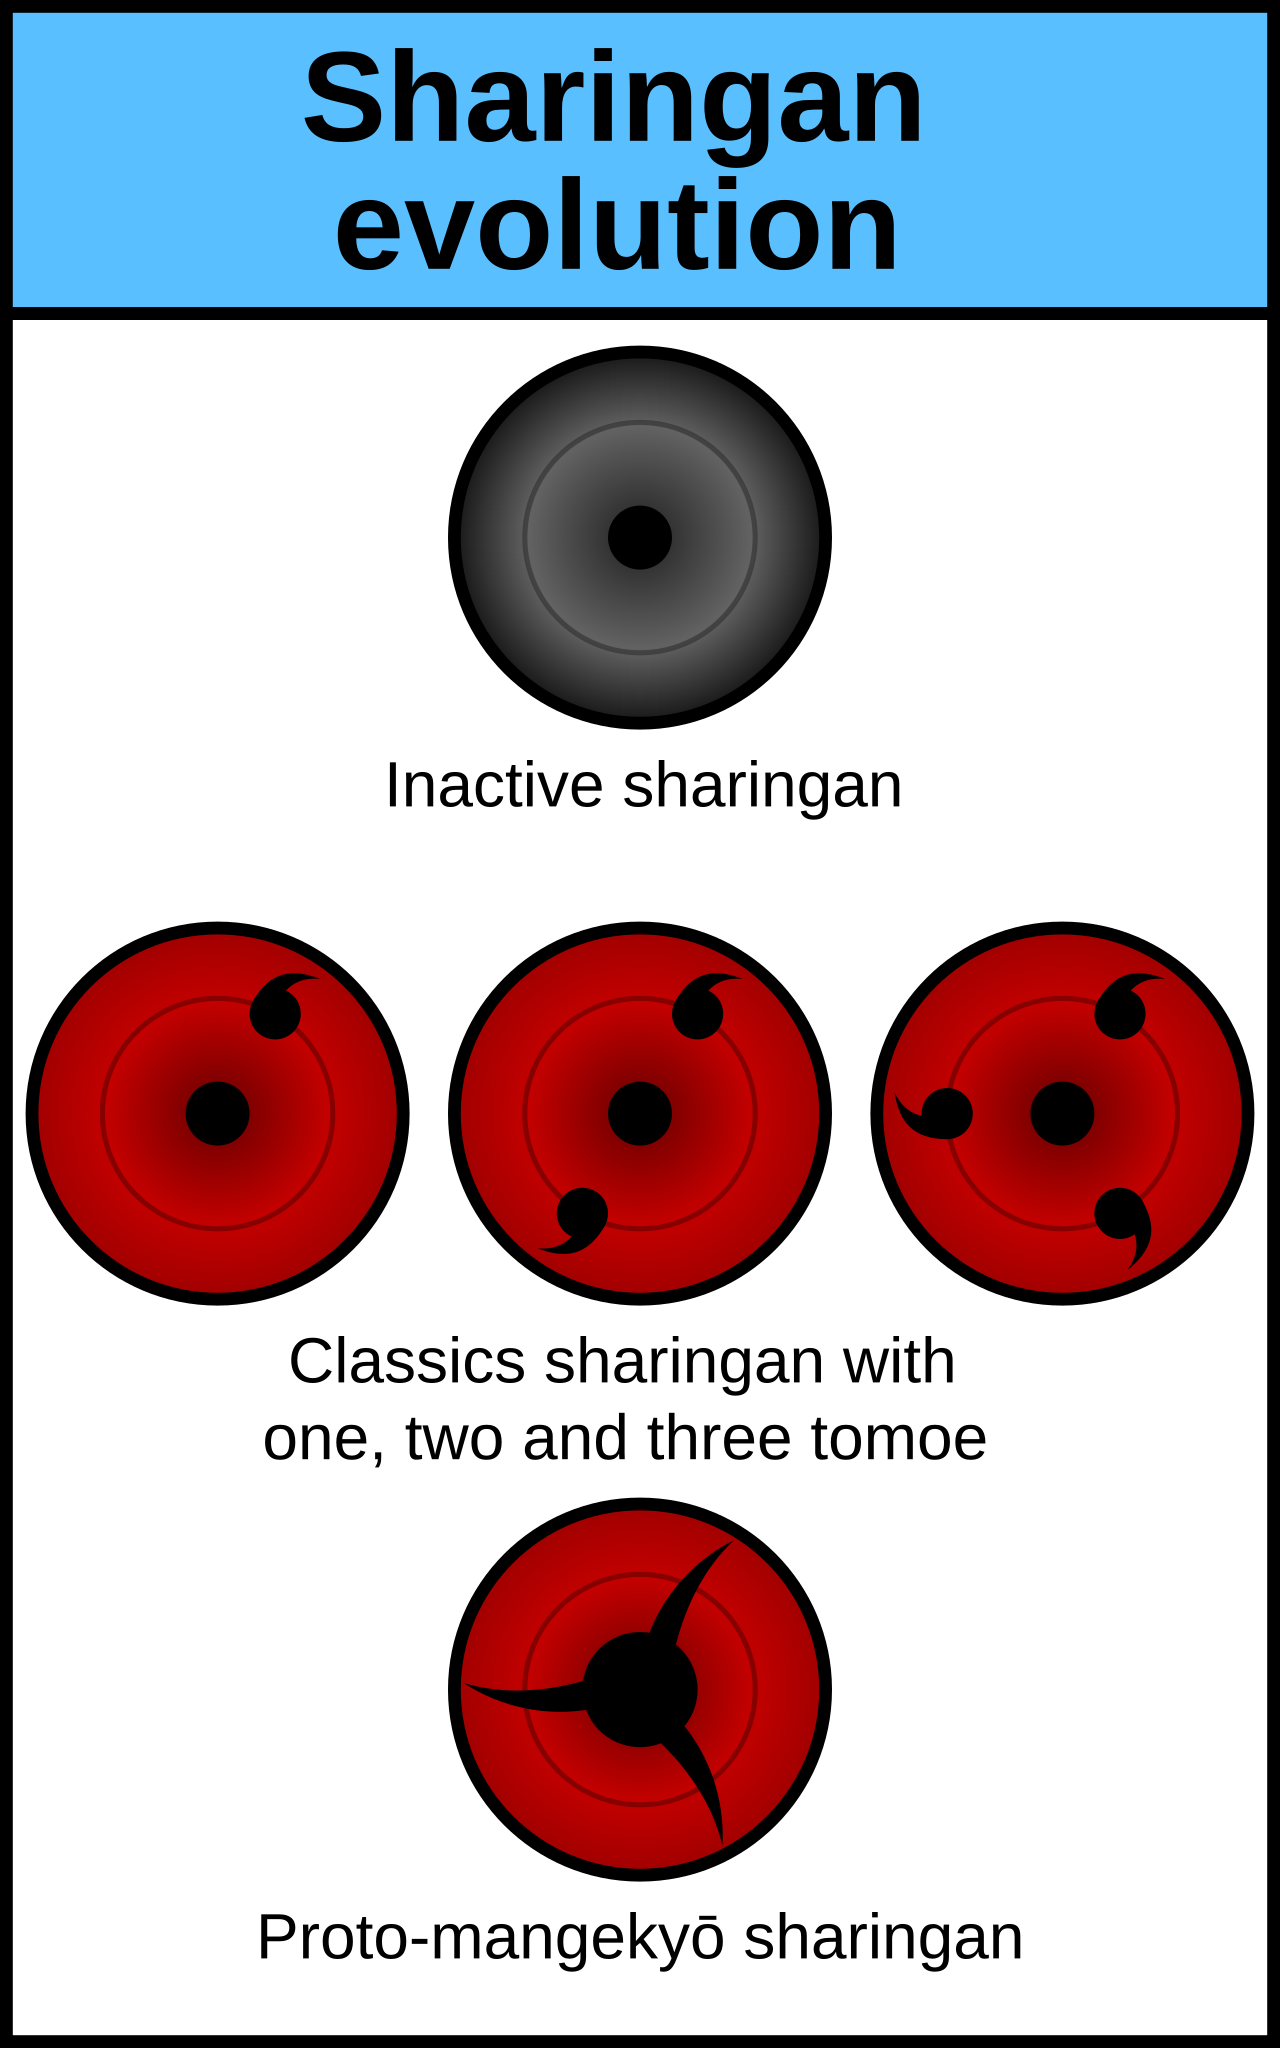
\includegraphics[width=0.7\linewidth]{../fig/Sharingan-evo.png} % Replace with the path to your image
    \caption{Sharingan}
    \label{fig:sharingan}
\end{figure}
\begin{figure}[H]
    \centering
    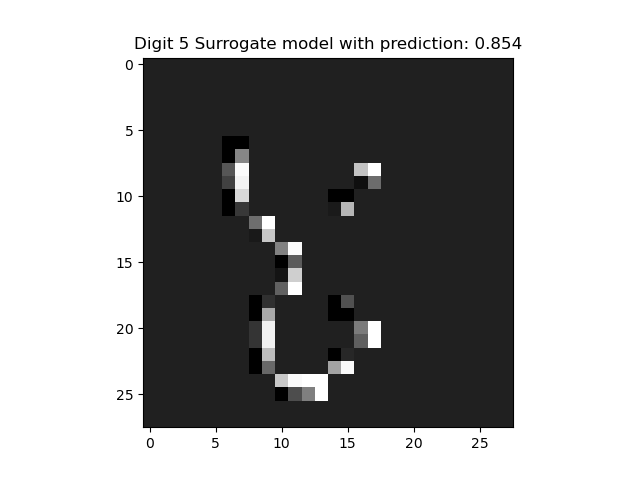
\includegraphics[width=0.7\linewidth]{../fig/ID 3-Digit 8 pred 5.png} % Replace with the path to your image
    \caption{Using conv2d and GAN}
    \label{fig:digit5}
\end{figure}


\section{Conclusion}
\ldots

\newpage
\begin{footnotesize} %%Makes bib footnotesize text size
\singlespacing %%Makes single spaced
\bibliographystyle{unsrt} %% Change to unsrt for ordered references
% \bibliographystyle{Phil_Review} %%bib style found in bst folder, in bibtex folder, in texmf folder.
\setlength{\bibsep}{5pt} %%Changes spacing between bib entries
\bibliography{Zotero} %%bib database found in bib folder, in bibtex folder
\thispagestyle{empty} %%Removes page numbers
\end{footnotesize} %%End makes bib small text size

\end{document}
